% ****** Start of file apssamp.tex ******
%
%   This file is part of the APS files in the REVTeX 4.2 distribution.
%   Version 4.2a of REVTeX, December 2014
%
%   Copyright (c) 2014 The American Physical Society.
%
%   See the REVTeX 4 README file for restrictions and more information.
%
% TeX'ing this file requires that you have AMS-LaTeX 2.0 installed
% as well as the rest of the prerequisites for REVTeX 4.2
%
% See the REVTeX 4 README file
% It also requires running BibTeX. The commands are as follows:
%
%  1)  latex apssamp.tex
%  2)  bibtex apssamp
%  3)  latex apssamp.tex
%  4)  latex apssamp.tex
%
\documentclass[%
 reprint,
%superscriptaddress,
%groupedaddress,
%unsortedaddress,
%runinaddress,
%frontmatterverbose, 
%preprint,
%preprintnumbers,
%nofootinbib,
%nobibnotes,
%bibnotes,
 amsmath,amssymb,
 aps,
%pra,
%prb,
%rmp,
%prstab,
%prstper,
%floatfix,
]{revtex4-2}
\usepackage{kotex}
\usepackage{graphicx}% Include figure files
\usepackage{dcolumn}% Align table columns on decimal point
\usepackage{bm}% bold math
\usepackage{chemformula}
\usepackage{chemfig}
\usepackage{setspace,supertabular}
\usepackage{longtable}
\usepackage{multirow}	
\usepackage{makecell}
\usepackage{amsmath}
%\usepackage{hyperref}% add hypertext capabilities
%\usepackage[mathlines]{lineno}% Enable numbering of text and display math
%\linenumbers\relax % Commence numbering lines

%\usepackage[showframe,%Uncomment any one of the following lines to test 
%%scale=0.7, marginratio={1:1, 2:3}, ignoreall,% default settings
%%text={7in,10in},centering,
%%margin=1.5in,
%%total={6.5in,8.75in}, top=1.2in, left=0.9in, includefoot,
%%height=10in,a5paper,hmargin={3cm,0.8in},
%]{geometry}

\begin{document}


\title{수소이야기 결과보고서}

\author{서울대학교 전기정보공학부 2018-12432 박정현}
 \email{alexist@snu.ac.kr}
\date{실험일자: 11/7/2023}% It is always \today, today,
             %  but any date may be explicitly specified

\begin{abstract}
본 실험에서는 
\end{abstract}

%\keywords{Suggested keywords}%Use showkeys class option if keyword
                              %display desired
\maketitle

%\tableofcontents

\section{\label{sec:level1}Assignment}
\subsection{\label{sec:level2}1}
보어의 원자모델은 20세기 초 수소원자의 방출스펙트럼을 설명하기 위해 제시되었다. 방출스펙트럼이 양자화되어 있음을 설명하기 위해 전자가 양성자를 돌 때 나타나는 각운동량을 $n\hbar$로 양자화한 뒤 전자가 양성자 주위를 타원궤도에서 공전함을 가정하여 주어지는 에너지가 양자화됬음을 제시하였다.

당시의 원자의 방출 스펙트럼을 설명할 수는 있었지만 전자가 가속하여 전자기파를 방출하면서 핵과 충돌하지 않는 원인을 제시하지 못하였다. 또한 이후에 발견된 fine structure, hyperfine structure와 같은 원자의 세밀한 구조를 설명하지 못한다는 한계점이 존재한다. 이를 해결하기 위해 슈뢰딩거 방정식을 통해 수소 원자를 풀어야만 하며 추가적으로 상대론적인 효과 또한 포함시켜야 세밀한 원자 구조를 정확히 풀어낼 수 있다.상대론을 고려하여 계산하는 경우 원자핵과 전자사이의 상호작용, 전자의 에너지가 상대론적으로 표현되는 것, 그리고 전자의 randomness(Darwin Term)에 의해 전자의 각운동량에 의해 축퇴화가 사라지게 된다.[2] 하지만 본 실험에서는 이러한 fine structure를 과측할 정도의 높은 resolution의 장비를 사용하지 않아 관측하지 못하므로 이러한 상대론적인 효과는 무시할 수 있다.

\subsection{\label{sec:level2}2}
\subsubsection{\label{sec:level3}a}
물의 전기분해할 때 전지를 통과한 전자들이 물을 통해 이동하여 반대편 전극에 도달하여야 한다. 순수한 물의 자동 이온화는 $K_{w} = 10\times10^{-14}$이므로 매우 적은 양의 이온들만이 존재한다. 따라서 이온화 정도가 매우큰 강산에 해당하는 \ch{H2SO4}수용액을 넣어 전류가 잘 통하게 만든다.

\subsubsection{\label{sec:level3}b}
물의 전기분해하는 화학반응식은 각각의 cathode, anode 전극에 대해서 아래와 같다.
\begin{align}
	\ch{2 H3O^{+}(aq) + 2 e-}&\ch{ -> H2(g) + 2 H2O(l)} \\
	\ch{3 H2O(l)} &\ch{-> 1/2  O2(g) + 2 H3O^{+}(aq) + 2 e-}
\end{align}
각각의 화학반응에 대한 전압은 아래와 같다.
\begin{align}
	\mathcal{E} &= \mathcal{E}^{o} - \frac{0.0592}{2}\log{\frac{P_{\ch{H2}}}{[\ch{H3O^{+}}]^{2}}}\\
	&=0 - \frac{0.0592}{2}\log{\frac{1}{(10^{-7})^{2}}}\\
	&= -0.414V
\end{align}

\begin{align}
	\mathcal{E} &= \mathcal{E}^{o} - \frac{0.0592}{2}\log{\frac{1}{P_{\ch{O2}}^{1/2}[\ch{H3O^{+}}]^{2}}}\\
	&=1.229 - \frac{0.0592}{2}\log{\frac{1}{(10^{-7})^{2}}} V \\
	&= 0.815 V
\end{align}

만약 anode에서 산화 전위가 0.815V보다 큰 경우 반응이 존재하고 anode에 가해지는 전압이 0.815V 부근인 경우 \ch{O2}가 먼저 산화되므로 반응은 일어나지 않는다. 마찬가지로 cathode에서 산화 전위가 -0.414V보다 작은 경우 \ch{H2}가 먼저 환원되므로 반응은 일어나지 않는다. Anode에서 \ch{SO2} gas가 발생하는 경우 반응은 아래와 같다.

\begin{align}
	\ch{SO4^{2-}(aq) -> SO2(g) + O2(g) + 2 e^{-}}
\end{align}

이 때 해당 반응의 반쪽 전지 전압은 아래와 같다.

\begin{align}
	\mathcal{E} &= \mathcal{E}^{o} - \frac{0.0592}{2}\log{\frac{P_{\ch{SO2}}P_{\ch{O2}}}{[\ch{SO4^{2-}}]}}
\end{align}

\ch{SO4^{2-}}의 농도가 매우 낮은 경우 $\mathcal{E}$값이 매우 커져 해당 \ch{SO2}기체는 발생하지 않는다. 하지만 \ch{SO4^{2-}}의 농도가 충분히 커 0.815 V보다 작아지는 경우 산소기체 대신 \ch{SO2}가 발생할 수 있을 것이다.[1]


\subsubsection{\label{sec:level3}c}
염소 이온이 염소 기체가 되는 반쪽 반응식과 해당하는 전압은 아래와 같다.
\begin{align}
	\ch{Cl^{-}(aq) -> 1/2 Cl2(g) + e^{-}}
\end{align}
\begin{align}
	\mathcal{E} &= \mathcal{E}^{o} - \frac{0.0592}{1}\log{\frac{[\ch{Cl^{-}}]}{P_{\ch{Cl2}}^{1/2}}}\\
	&=1.36 - 0.0592\log{[\ch{Cl^{-}}]} V
\end{align}
\ch{Cl^{-}}의 농도가 1M임을 가정해도 1.36V의 반쪽 전지 전압을 가지므로 염소기체는 산소보다 환원되려는 성질이 크므로 anode에 가해지는 전압이 0.815V이상이고 1.36V 이하이면 큰 문제가 없다. 하지만 1.36V보다 충분히 큰 전압이 가해지거나 \ch{Cl-}의 농도가 매우 커져 log항을 무시할 수 없는 경우 \ch{Cl-}의 산화가 활발하게 발생하므로 \ch{Cl2}기체가 발생하게 된다. 따라서 이론적으로는 염소기체의 발생을 조절할 수 있으나 안전을 위해 되도록 사용하지 않는것이 좋다.[1]

\section{\label{sec:level1}Data \& Results}
\subsection{\label{sec:level2}금속 원소의 당량 결정}
각 금속과의 반응에서 생성된 기체의 양은 Tab.\ref{tab:gengas}와 같다.

\begin{table}[h]
\caption{\label{tab:gengas} 금속 질량 및 생성된 기체 부피}
\begin{tabular}{l|c|c} \hline \hline
금속 & 금속 질량[mg] & 생성된 기체 부피 [mL] \\ \hline
\ch{Zn} & $67\pm1$ & $34.2 \pm 0.3 $ \\
\ch{Mg} & $55\pm1$ & $52.5 \pm 0.3 $ \\
\ch{Al} & $51\pm1$ & $78.5 \pm 0.3 $ \\ \hline \hline 
\end{tabular}
\end{table}

수소가 이상기체임을 가정하면 각 원소별 반응한 수소의 몰수는 $n = \frac{2PV}{RT}$로 계산된다. 금속의 당량은 원자량을 금속의 산화수로 계산되므로 각 원소별 화학반응식은 아래와 같으므로 각 원소별 당량은 아래와 같다.
\begin{align}
	\ch{Zn(s) + 2HCl(aq) ->ZnCl2(aq) + H2(g)}
\end{align}
\begin{align}
	\ch{Mg(s) + 2HCl(aq) ->MgCl2(aq) + H2(g)}
\end{align}
\begin{align}
	\ch{2Al(s) + 6HCl(aq) ->2AlCl3(aq) + 3H2(g)}
\end{align}

\begin{table}[h]
\caption{\label{tab:dang} 각 금속별 당량}
\begin{tabular}{l|c|c|c|c} \hline \hline
\multirowcell{2}{금속} & 반응한 수소 & 측정된 & 이론적 &\multirowcell{2}{오차} \\ 
& 몰수[mol] & 당량[g/eq] & 당량 [g/eq] &\\ \hline
\ch{Zn} & $(2.78\pm0.01)\times10^{-3}$ & $24.1 \pm 0.2 $ & 32.69 & 26.2\% \\
\ch{Mg} & $(4.26\pm0.01)\times10^{-3}$ & $12.9 \pm 0.3 $ & 12.15  & 6.13\% \\
\ch{Al} & $(6.38\pm0.01)\times10^{-3}$ & $8.00 \pm 0.1 $ & 9.00 & 11.1\% \\ \hline \hline 
\end{tabular}
\end{table}

\subsection{\label{sec:level2}원소들의 스펙트럼}
\subsubsection{\label{sec:level3}중수소}
중수소는 수소와 동일하나 원자핵에 중성자가 하나 더 존재한다. 고전적으로 계산한 보어 원자의 에너지 준위는 아래와 같다.

\begin{align}
	E_{n} &= \frac{me^{4}}{(4\pi\varepsilon_{0})^{2}2\hbar^{2}}\frac{1}{n^{2}}
\end{align}

수소의 에너지를 계산할 때 원자 핵은 고정된 상태로 계산하였다. 하지만 실제로는 원자핵 또한 미세하게 움직이고 있다. 따라서 에너지는 전자의 질량이 아닌 전자와 원자핵의 질량을 모두 고려한 환산 질량 $\mu$을 대입해야 한다.

\begin{align}
	\mu &= \frac{Mm}{M+m}\\
	&\simeq m\left( 1- \frac{m}{M} \right)
\end{align}

환산질량을 대입하면 수소는 $m/M$만큼 감소한 주파수가 측정될 것이고 중수소는 $m/2M$만큼 감소한 주파수가 관측될 것이다. 본 실험에서 사용한 관측 장비에서 $m/2M \simeq 1/1800$만큼의 차이는 측정할 수 없으므로 관측되는 스펙트럼은 수소와 동일할 것이다. 실제로 실험 결과 4개의 스펙트럼 피크가 확인 되었는데 각각 적색, 하늘색, 파란색, 보라색이 관측되었다. 각각 Tab.\ref{tab:deutro}의 이론적인 예측과 동일함을 알 수 있다.

\begin{table}[h]
\caption{\label{tab:deutro} 중수소 스펙트럼}
\begin{tabular}{l|c|c} \hline \hline
에너지 준위 & 파장[nm] & 색 \\ \hline
\ch{3->2} & 656 & 적색 \\ 
\ch{4->2} & 486 & 하늘색 \\ 
\ch{5->2} & 434 & 청색 \\ 
\ch{6->2} & 410 & 보라색 \\ \hline \hline 
\end{tabular}
\end{table}

\subsubsection{\label{sec:level3}수은}
수은의 energy diagram은 Fig.\ref{fig:Hg}와 같다.[4] 각각의 에너지 레벨은 $n^{2S+1}L_{H}$로 표현되었는데 2S+1은 전자스핀에 의한 muliplicity, L은 궤도각운동량, J는 총 각운동량, 그리고 n은 에너지 레벨로 전자와 핵 사이의 상호작용과 같은 상대론적인 효과를 모두 고려한 energy level을 표현하는 term symbol이다.[3] 다이어그램에서 알 수 있듯 동일한 주양자수임에도 불구하고 다른 에너지 레벨을 가짐을 확인할 수 있다. 실험에서 약 3개의 스펙트럼 피크가 관측되었는데 각각 아래의 전자전이에 해당함을 알 수 있다.

\begin{figure}[htbp]
	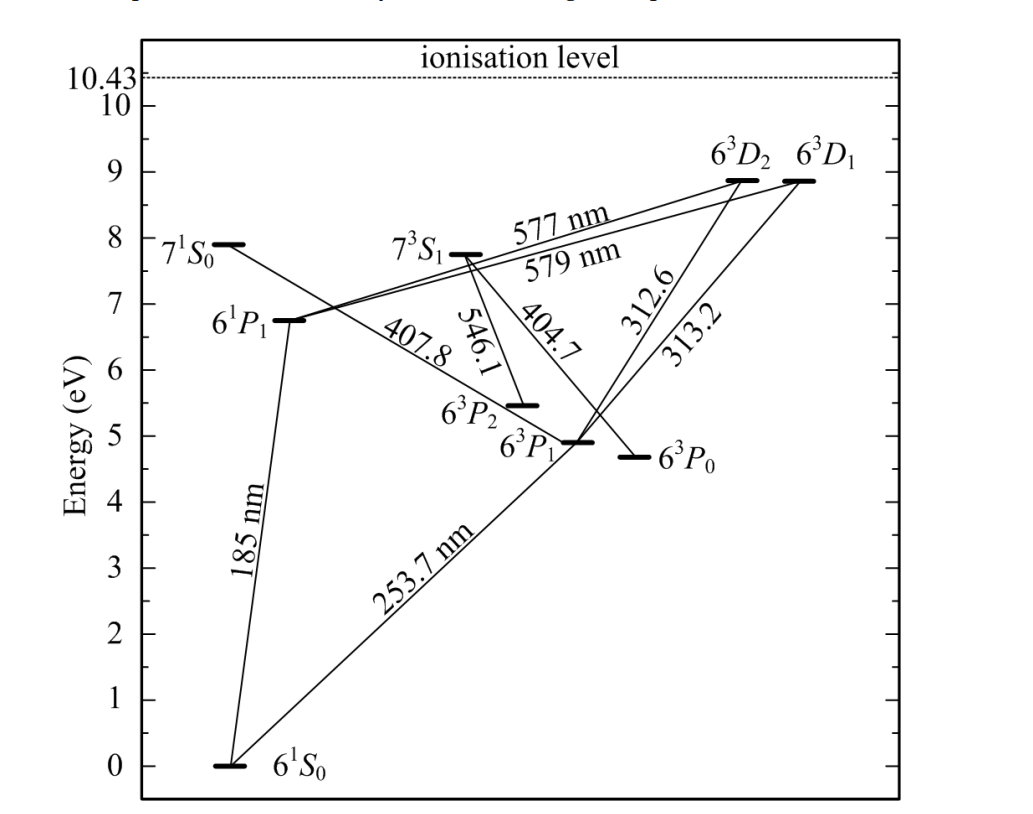
\includegraphics[width = 0.9\linewidth]{Hg.png}% Here is how to import EPS art
	\caption{\label{fig:Hg} 수은 에너지 레벨}
\end{figure}

\begin{table}[h]
\caption{\label{tab:mercury} 수은 스펙트럼}
\begin{tabular}{l|c|c} \hline \hline
에너지 준위 & 파장[nm] & 색 \\ \hline
$6^{3}D\rightarrow 6^{1}P_{1}$ & 577-579 & 연두색 \\ \hline
$7^{3}S_{1}\rightarrow 6^{3}P_{2}$ & 546.1 & 노란색 \\ \hline
$7^{3}S_{1}\rightarrow 6^{3}P_{0}$ & \multirowcell{2}{404-408} & \multirowcell{2}{보라색} \\ 
$7^{1}S_{0}\rightarrow 6^{3}P_{1}$ & & \\  \hline \hline 
\end{tabular}
\end{table}

\subsubsection{\label{sec:level3}헬륨}
헬륨의 에너지 레벨은 Fig.\ref{fig:He}와 같다. 약 3개의 스펙트럼 피크가 관측되었는데 각각 아래의 전자 전이에 해당함을 알 수 있다.

\begin{figure}[htbp]
	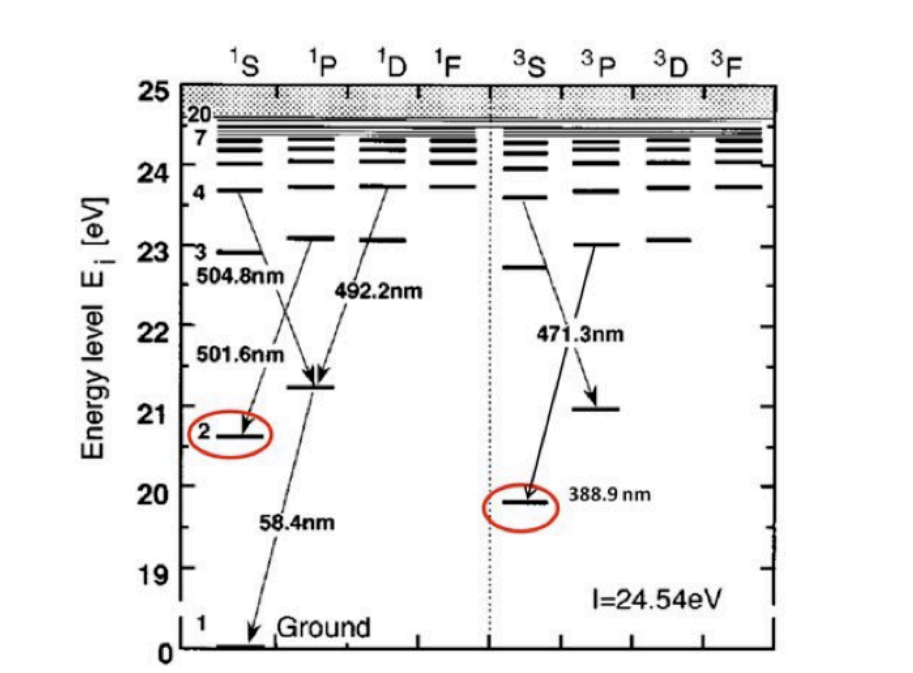
\includegraphics[width = 0.9\linewidth]{He.png}% Here is how to import EPS art
	\caption{\label{fig:He} 헬륨 에너지 레벨}
\end{figure}

\begin{table}[h]
\caption{\label{tab:helium} 헬륨 스펙트럼}
\begin{tabular}{l|c|c} \hline \hline
에너지 준위 & 파장[nm] & 색 \\ \hline
$4^{1}S\rightarrow 2^{1}P$ & \multirowcell{3}{490-505} & \multirowcell{3}{하늘색} \\ 
$3^{1}P\rightarrow 2^{1}S$ & & \\  
$4^{3}S\rightarrow 3^{3}P$ & & \\  \hline
$4^{3}S\rightarrow 4^{3}P$ & 471.3 & 파란색 \\ \hline
$3^{3}P\rightarrow 2^{3}S$ & 388.9 & 보라색 \\ \hline\hline \hline 
\end{tabular}
\end{table}

\subsubsection{\label{sec:level3}아르곤}
아르곤의 방출 스펙트럼은 Fig.\ref{fig:Ar}으로 알려져 있다.[6] 실험에서 약 4개의 스펙트럼 피크가 각각 20nm의 파장 차이 내에 해당하는 피크에 해당함을 알 수 있다.

\begin{figure}[htbp]
	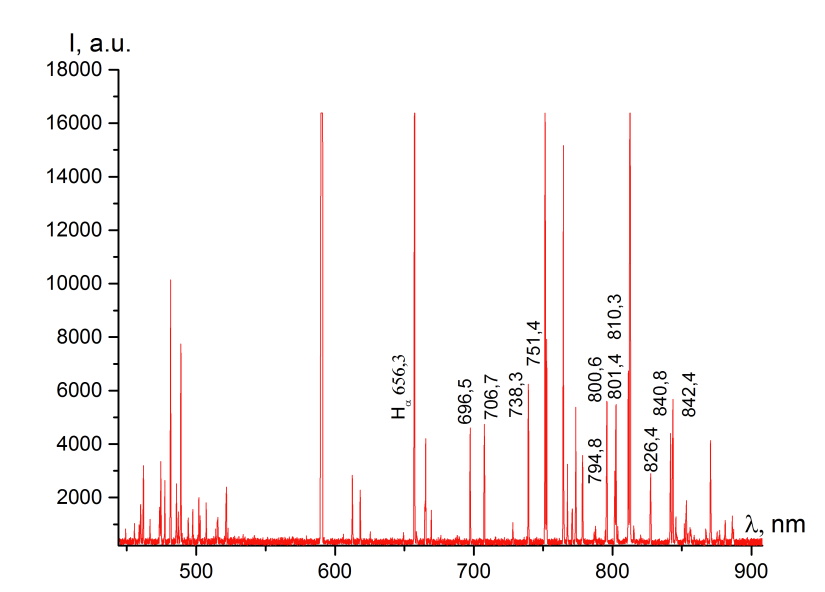
\includegraphics[width = 0.9\linewidth]{Ar.png}% Here is how to import EPS art
	\caption{\label{fig:Ar} 아르곤 방출 스펙트럼}
\end{figure}

\subsection{\label{sec:level2}물의 전기분해}
Anode에는 5mL, cathode에는 10mL의 기체가 포집되었다. 이를 통해 anode에서는 산소, cathode에서는 수소 기체가 발생함을 화인하였다.

\section{\label{sec:level1}Conclusion \& Discussion}
수소를 비눗방울에 포집하기 어려웠다. 조금 더 포집을 쉽게 하기 위해 수상치환을 통해 수소를 포집한 이후 비눗방울을 만들면 더 원활한 실험이 가능할 것이다.

아연과 알루미늄의 경우 예상한 당량보다 낮은 당량이 측정되었다. 이것은 반응이 끝나기까지 충분한 시간을 기다리지 않아 발생한 것으로 결론지었다. 특히 알루미늄의 경우 반응시간이 매우 길고 반응이 끝났는지 확인하는데 어려움이 있었다. 또한 반응 이후 대기압과 플라스크 내의 압력이 동일하지 않으므로 $n = PV/RT$에서 더 높은 압력을 대입해야 할 것이다. 압력을 모두 고려하는 경우 더 정확한 당량을 측정할 수 있을 것이다. 마그네슘의 경우 이론적으로 예측한 당량보다 높은 값이 측정되었는데 이것은 초기 메스플라스크에 남아있던 공기방울, 그리고 마게를 덮으면서 흘러들어간 공기, 그리고 메스플라스크의 부피를 측정할 때 나타난 오차로 인해 발생한 것으로 결론지었다.

실제 수소의 스펙트럼과 중수소의 스펙트럼이 이론적으로 일치하는지 수치적으로 확인할 수 어려웠다. 이를 해결하기 위해 더 높은 해상도의 스펙트로스코피를 이용해 중수소와 수소의 스펙트럼을 측정하면 앞서 이론적으로 예측한 스펙트럼이 일치하는 것을 확인할 수 있을 것이다. 또한 fine structure 또한 측정이 가능할 것이다.

\section{\label{sec:level1}Reference}
[1] Oxtoby, D., Gillis, H., \& Campion, A. (2007, April 2). Equilibrium in Chemical Reactions. In \textit{Principles of Modern Chemistry} (6th ed., pp. 735-737). Cengage Learning.

[2] CJ FOOT 원자물리 fine structure

[3] CJ FOOT 원자물리 term symbol

[4] Symmetrization and Amplification of Germicidal Radiation Flux Produced by a Mercury Amalgam UV Lamp in Cylindrical Cavity with Diffusely Reflective Walls

[5] Plasma Assisted Cleaning by Metastable-Atom Neutralization (PACMAN) A Plasma Approach to Cleanliness in Lithography

[6] OPTICAL EMISSION SPECTROSCOPY OF MAGNETHRON DISCHARGE Ar/Cu PLASMA

\end{document}
%
% ****** End of file apssamp.tex ******
